\documentclass[1p]{elsarticle_modified}
%\bibliographystyle{elsarticle-num}

%\usepackage[colorlinks]{hyperref}
%\usepackage{abbrmath_seonhwa} %\Abb, \Ascr, \Acal ,\Abf, \Afrak
\usepackage{amsfonts}
\usepackage{amssymb}
\usepackage{amsmath}
\usepackage{amsthm}
\usepackage{scalefnt}
\usepackage{amsbsy}
\usepackage{kotex}
\usepackage{caption}
\usepackage{subfig}
\usepackage{color}
\usepackage{graphicx}
\usepackage{xcolor} %% white, black, red, green, blue, cyan, magenta, yellow
\usepackage{float}
\usepackage{setspace}
\usepackage{hyperref}

\usepackage{tikz}
\usetikzlibrary{arrows}

\usepackage{multirow}
\usepackage{array} % fixed length table
\usepackage{hhline}

%%%%%%%%%%%%%%%%%%%%%
\makeatletter
\renewcommand*\env@matrix[1][\arraystretch]{%
	\edef\arraystretch{#1}%
	\hskip -\arraycolsep
	\let\@ifnextchar\new@ifnextchar
	\array{*\c@MaxMatrixCols c}}
\makeatother %https://tex.stackexchange.com/questions/14071/how-can-i-increase-the-line-spacing-in-a-matrix
%%%%%%%%%%%%%%%

\usepackage[normalem]{ulem}

\newcommand{\msout}[1]{\ifmmode\text{\sout{\ensuremath{#1}}}\else\sout{#1}\fi}
%SOURCE: \msout is \stkout macro in https://tex.stackexchange.com/questions/20609/strikeout-in-math-mode

\newcommand{\cancel}[1]{
	\ifmmode
	{\color{red}\msout{#1}}
	\else
	{\color{red}\sout{#1}}
	\fi
}

\newcommand{\add}[1]{
	{\color{blue}\uwave{#1}}
}

\newcommand{\replace}[2]{
	\ifmmode
	{\color{red}\msout{#1}}{\color{blue}\uwave{#2}}
	\else
	{\color{red}\sout{#1}}{\color{blue}\uwave{#2}}
	\fi
}

\newcommand{\Sol}{\mathcal{S}} %segment
\newcommand{\D}{D} %diagram
\newcommand{\A}{\mathcal{A}} %arc


%%%%%%%%%%%%%%%%%%%%%%%%%%%%%5 test

\def\sl{\operatorname{\textup{SL}}(2,\Cbb)}
\def\psl{\operatorname{\textup{PSL}}(2,\Cbb)}
\def\quan{\mkern 1mu \triangleright \mkern 1mu}

\theoremstyle{definition}
\newtheorem{thm}{Theorem}[section]
\newtheorem{prop}[thm]{Proposition}
\newtheorem{lem}[thm]{Lemma}
\newtheorem{ques}[thm]{Question}
\newtheorem{cor}[thm]{Corollary}
\newtheorem{defn}[thm]{Definition}
\newtheorem{exam}[thm]{Example}
\newtheorem{rmk}[thm]{Remark}
\newtheorem{alg}[thm]{Algorithm}

\newcommand{\I}{\sqrt{-1}}
\begin{document}

%\begin{frontmatter}
%
%\title{Boundary parabolic representations of knots up to 8 crossings}
%
%%% Group authors per affiliation:
%\author{Yunhi Cho} 
%\address{Department of Mathematics, University of Seoul, Seoul, Korea}
%\ead{yhcho@uos.ac.kr}
%
%
%\author{Seonhwa Kim} %\fnref{s_kim}}
%\address{Center for Geometry and Physics, Institute for Basic Science, Pohang, 37673, Korea}
%\ead{ryeona17@ibs.re.kr}
%
%\author{Hyuk Kim}
%\address{Department of Mathematical Sciences, Seoul National University, Seoul 08826, Korea}
%\ead{hyukkim@snu.ac.kr}
%
%\author{Seokbeom Yoon}
%\address{Department of Mathematical Sciences, Seoul National University, Seoul, 08826,  Korea}
%\ead{sbyoon15@snu.ac.kr}
%
%\begin{abstract}
%We find all boundary parabolic representation of knots up to 8 crossings.
%
%\end{abstract}
%\begin{keyword}
%    \MSC[2010] 57M25 
%\end{keyword}
%
%\end{frontmatter}

%\linenumbers
%\tableofcontents
%
\newcommand\colored[1]{\textcolor{white}{\rule[-0.35ex]{0.8em}{1.4ex}}\kern-0.8em\color{red} #1}%
%\newcommand\colored[1]{\textcolor{white}{ #1}\kern-2.17ex	\textcolor{white}{ #1}\kern-1.81ex	\textcolor{white}{ #1}\kern-2.15ex\color{red}#1	}

{\Large $\underline{12a_{0638}~(K12a_{0638})}$}

\setlength{\tabcolsep}{10pt}
\renewcommand{\arraystretch}{1.6}
\vspace{1cm}\begin{tabular}{m{100pt}>{\centering\arraybackslash}m{274pt}}
\multirow{5}{120pt}{
	\centering
	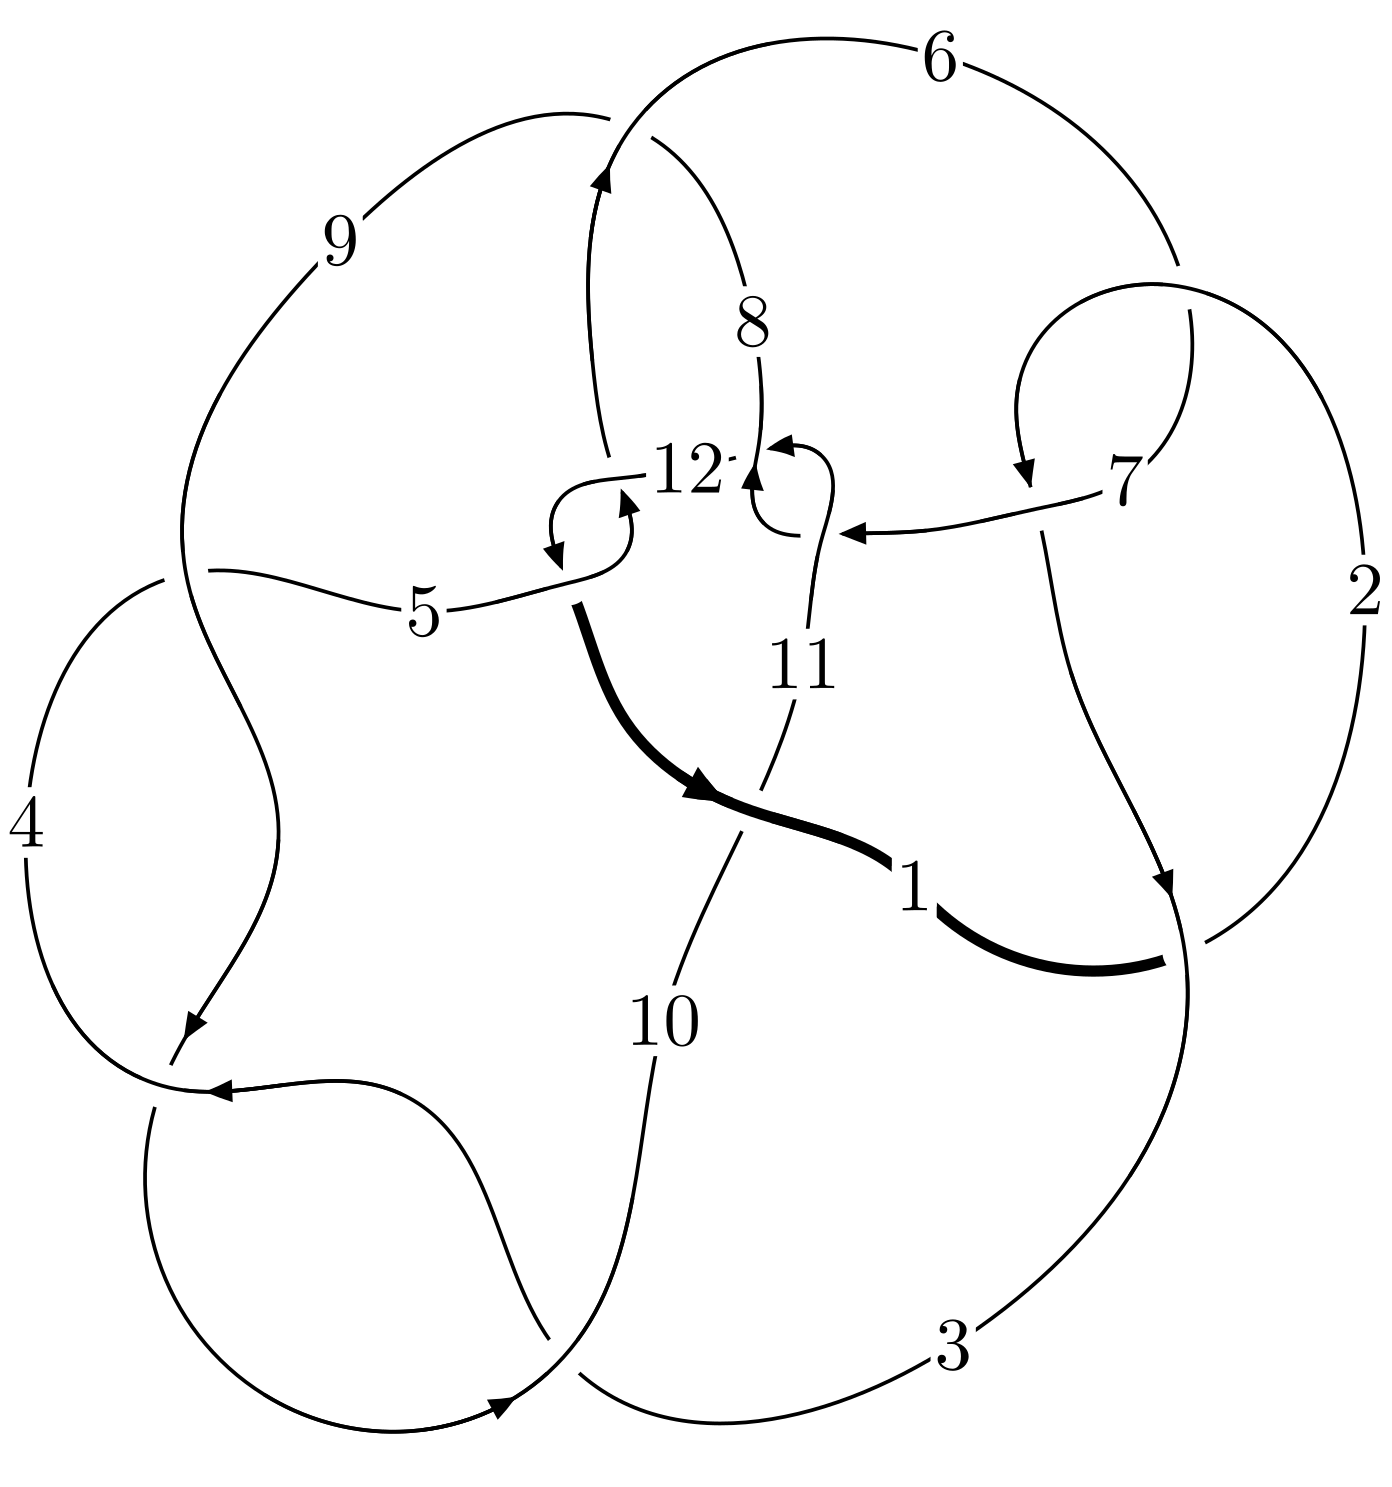
\includegraphics[width=112pt]{../../../GIT/diagram.site/Diagrams/png/1439_12a_0638.png}\\
\ \ \ A knot diagram\footnotemark}&
\allowdisplaybreaks
\textbf{Linearized knot diagam} \\
\cline{2-2}
 &
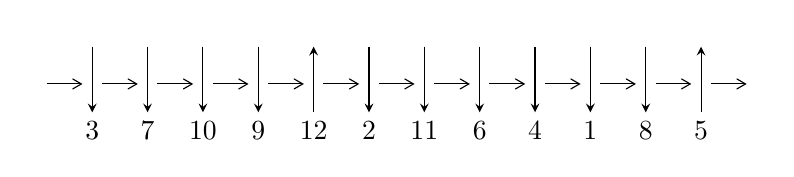
\begin{tikzpicture}[x=20pt, y=17pt]
	% nodes
	\node (C0) at (0, 0) {};
	\node (C1) at (1, 0) {};
	\node (C1U) at (1, +1) {};
	\node (C1D) at (1, -1) {3};

	\node (C2) at (2, 0) {};
	\node (C2U) at (2, +1) {};
	\node (C2D) at (2, -1) {7};

	\node (C3) at (3, 0) {};
	\node (C3U) at (3, +1) {};
	\node (C3D) at (3, -1) {10};

	\node (C4) at (4, 0) {};
	\node (C4U) at (4, +1) {};
	\node (C4D) at (4, -1) {9};

	\node (C5) at (5, 0) {};
	\node (C5U) at (5, +1) {};
	\node (C5D) at (5, -1) {12};

	\node (C6) at (6, 0) {};
	\node (C6U) at (6, +1) {};
	\node (C6D) at (6, -1) {2};

	\node (C7) at (7, 0) {};
	\node (C7U) at (7, +1) {};
	\node (C7D) at (7, -1) {11};

	\node (C8) at (8, 0) {};
	\node (C8U) at (8, +1) {};
	\node (C8D) at (8, -1) {6};

	\node (C9) at (9, 0) {};
	\node (C9U) at (9, +1) {};
	\node (C9D) at (9, -1) {4};

	\node (C10) at (10, 0) {};
	\node (C10U) at (10, +1) {};
	\node (C10D) at (10, -1) {1};

	\node (C11) at (11, 0) {};
	\node (C11U) at (11, +1) {};
	\node (C11D) at (11, -1) {8};

	\node (C12) at (12, 0) {};
	\node (C12U) at (12, +1) {};
	\node (C12D) at (12, -1) {5};
	\node (C13) at (13, 0) {};

	% arrows
	\draw[->,>={angle 60}]
	(C0) edge (C1) (C1) edge (C2) (C2) edge (C3) (C3) edge (C4) (C4) edge (C5) (C5) edge (C6) (C6) edge (C7) (C7) edge (C8) (C8) edge (C9) (C9) edge (C10) (C10) edge (C11) (C11) edge (C12) (C12) edge (C13) ;	\draw[->,>=stealth]
	(C1U) edge (C1D) (C2U) edge (C2D) (C3U) edge (C3D) (C4U) edge (C4D) (C5D) edge (C5U) (C6U) edge (C6D) (C7U) edge (C7D) (C8U) edge (C8D) (C9U) edge (C9D) (C10U) edge (C10D) (C11U) edge (C11D) (C12D) edge (C12U) ;
	\end{tikzpicture} \\
\hhline{~~} \\& 
\textbf{Solving Sequence} \\ \cline{2-2} 
 &
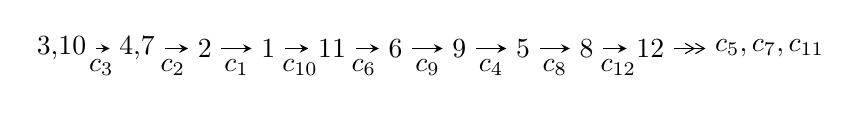
\begin{tikzpicture}[x=23pt, y=7pt]
	% node
	\node (A0) at (-1/8, 0) {3,10};
	\node (A1) at (17/16, 0) {4,7};
	\node (A2) at (17/8, 0) {2};
	\node (A3) at (25/8, 0) {1};
	\node (A4) at (33/8, 0) {11};
	\node (A5) at (41/8, 0) {6};
	\node (A6) at (49/8, 0) {9};
	\node (A7) at (57/8, 0) {5};
	\node (A8) at (65/8, 0) {8};
	\node (A9) at (73/8, 0) {12};
	\node (C1) at (1/2, -1) {$c_{3}$};
	\node (C2) at (13/8, -1) {$c_{2}$};
	\node (C3) at (21/8, -1) {$c_{1}$};
	\node (C4) at (29/8, -1) {$c_{10}$};
	\node (C5) at (37/8, -1) {$c_{6}$};
	\node (C6) at (45/8, -1) {$c_{9}$};
	\node (C7) at (53/8, -1) {$c_{4}$};
	\node (C8) at (61/8, -1) {$c_{8}$};
	\node (C9) at (69/8, -1) {$c_{12}$};
	\node (A10) at (11, 0) {$c_{5},c_{7},c_{11}$};

	% edge
	\draw[->,>=stealth]	
	(A0) edge (A1) (A1) edge (A2) (A2) edge (A3) (A3) edge (A4) (A4) edge (A5) (A5) edge (A6) (A6) edge (A7) (A7) edge (A8) (A8) edge (A9) ;
	\draw[->>,>={angle 60}]	
	(A9) edge (A10);
\end{tikzpicture} \\ 

\end{tabular} \\

\footnotetext{
The image of knot diagram is generated by the software ``\textbf{Draw programme}" developed by Andrew Bartholomew(\url{http://www.layer8.co.uk/maths/draw/index.htm\#Running-draw}), where we modified some parts for our purpose(\url{https://github.com/CATsTAILs/LinksPainter}).
}\phantom \\ \newline 
\centering \textbf{Ideals for irreducible components\footnotemark of $X_{\text{par}}$} 
 
\begin{align*}
I^u_{1}&=\langle 
-3.88047\times10^{205} u^{89}+4.82669\times10^{205} u^{88}+\cdots+8.17391\times10^{204} b+1.54211\times10^{206},\\
\phantom{I^u_{1}}&\phantom{= \langle  }2.69752\times10^{206} u^{89}-3.08673\times10^{206} u^{88}+\cdots+8.17391\times10^{204} a-1.57877\times10^{207},\;u^{90}- u^{89}+\cdots-13 u-1\rangle \\
\\
\end{align*}
\raggedright * 1 irreducible components of $\dim_{\mathbb{C}}=0$, with total 90 representations.\\
\footnotetext{All coefficients of polynomials are rational numbers. But the coefficients are sometimes approximated in decimal forms when there is not enough margin.}
\newpage
\renewcommand{\arraystretch}{1}
\centering \section*{I. $I^u_{1}= \langle -3.88\times10^{205} u^{89}+4.83\times10^{205} u^{88}+\cdots+8.17\times10^{204} b+1.54\times10^{206},\;2.70\times10^{206} u^{89}-3.09\times10^{206} u^{88}+\cdots+8.17\times10^{204} a-1.58\times10^{207},\;u^{90}- u^{89}+\cdots-13 u-1 \rangle$}
\flushleft \textbf{(i) Arc colorings}\\
\begin{tabular}{m{7pt} m{180pt} m{7pt} m{180pt} }
\flushright $a_{3}=$&$\begin{pmatrix}1\\0\end{pmatrix}$ \\
\flushright $a_{10}=$&$\begin{pmatrix}0\\u\end{pmatrix}$ \\
\flushright $a_{4}=$&$\begin{pmatrix}1\\u^2\end{pmatrix}$ \\
\flushright $a_{7}=$&$\begin{pmatrix}-33.0016 u^{89}+37.7631 u^{88}+\cdots+1468.09 u+193.147\\4.74738 u^{89}-5.90500 u^{88}+\cdots-173.610 u-18.8662\end{pmatrix}$ \\
\flushright $a_{2}=$&$\begin{pmatrix}-8.45664 u^{89}+11.0243 u^{88}+\cdots+256.917 u+9.20347\\-6.17248 u^{89}+7.40897 u^{88}+\cdots+257.954 u+31.5861\end{pmatrix}$ \\
\flushright $a_{1}=$&$\begin{pmatrix}-14.6291 u^{89}+18.4333 u^{88}+\cdots+514.871 u+40.7896\\-6.17248 u^{89}+7.40897 u^{88}+\cdots+257.954 u+31.5861\end{pmatrix}$ \\
\flushright $a_{11}=$&$\begin{pmatrix}17.7342 u^{89}-28.6739 u^{88}+\cdots-80.1654 u+48.2554\\10.8888 u^{89}-13.4259 u^{88}+\cdots-401.828 u-45.1321\end{pmatrix}$ \\
\flushright $a_{6}=$&$\begin{pmatrix}-23.5669 u^{89}+26.3603 u^{88}+\cdots+1121.51 u+150.471\\-0.908820 u^{89}+0.780287 u^{88}+\cdots+61.0914 u+11.0352\end{pmatrix}$ \\
\flushright $a_{9}=$&$\begin{pmatrix}u\\u^3+u\end{pmatrix}$ \\
\flushright $a_{5}=$&$\begin{pmatrix}u^2+1\\u^4+2 u^2\end{pmatrix}$ \\
\flushright $a_{8}=$&$\begin{pmatrix}-10.0388 u^{89}+4.07039 u^{88}+\cdots+1067.53 u+183.313\\9.64910 u^{89}-12.1029 u^{88}+\cdots-343.266 u-36.0497\end{pmatrix}$ \\
\flushright $a_{12}=$&$\begin{pmatrix}-9.59366 u^{89}+12.3295 u^{88}+\cdots+310.049 u+14.7507\\-5.77007 u^{89}+6.89531 u^{88}+\cdots+241.600 u+29.5670\end{pmatrix}$\\&\end{tabular}
\flushleft \textbf{(ii) Obstruction class $= -1$}\\~\\
\flushleft \textbf{(iii) Cusp Shapes $= 31.5469 u^{89}-41.0990 u^{88}+\cdots-989.110 u-113.884$}\\~\\
\newpage\renewcommand{\arraystretch}{1}
\flushleft \textbf{(iv) u-Polynomials at the component}\newline \\
\begin{tabular}{m{50pt}|m{274pt}}
Crossings & \hspace{64pt}u-Polynomials at each crossing \\
\hline $$\begin{aligned}c_{1}\end{aligned}$$&$\begin{aligned}
&u^{90}+35 u^{89}+\cdots+223 u+9
\end{aligned}$\\
\hline $$\begin{aligned}c_{2},c_{6}\end{aligned}$$&$\begin{aligned}
&u^{90}-3 u^{89}+\cdots-19 u+3
\end{aligned}$\\
\hline $$\begin{aligned}c_{3},c_{4},c_{9}\end{aligned}$$&$\begin{aligned}
&u^{90}+u^{89}+\cdots+13 u-1
\end{aligned}$\\
\hline $$\begin{aligned}c_{5},c_{12}\end{aligned}$$&$\begin{aligned}
&u^{90}-3 u^{89}+\cdots-19 u+3
\end{aligned}$\\
\hline $$\begin{aligned}c_{7},c_{11}\end{aligned}$$&$\begin{aligned}
&u^{90}+u^{89}+\cdots-17 u-1
\end{aligned}$\\
\hline $$\begin{aligned}c_{8}\end{aligned}$$&$\begin{aligned}
&1089(1089 u^{90}+7095 u^{89}+\cdots+166909 u-7597)
\end{aligned}$\\
\hline $$\begin{aligned}c_{10}\end{aligned}$$&$\begin{aligned}
&1089(1089 u^{90}+5709 u^{89}+\cdots+497255 u+37873)
\end{aligned}$\\
\hline
\end{tabular}\\~\\
\newpage\renewcommand{\arraystretch}{1}
\flushleft \textbf{(v) Riley Polynomials at the component}\newline \\
\begin{tabular}{m{50pt}|m{274pt}}
Crossings & \hspace{64pt}Riley Polynomials at each crossing \\
\hline $$\begin{aligned}c_{1}\end{aligned}$$&$\begin{aligned}
&y^{90}+41 y^{89}+\cdots+119237 y+81
\end{aligned}$\\
\hline $$\begin{aligned}c_{2},c_{6}\end{aligned}$$&$\begin{aligned}
&y^{90}-35 y^{89}+\cdots-223 y+9
\end{aligned}$\\
\hline $$\begin{aligned}c_{3},c_{4},c_{9}\end{aligned}$$&$\begin{aligned}
&y^{90}+89 y^{89}+\cdots-83 y+1
\end{aligned}$\\
\hline $$\begin{aligned}c_{5},c_{12}\end{aligned}$$&$\begin{aligned}
&y^{90}+57 y^{89}+\cdots+65 y+9
\end{aligned}$\\
\hline $$\begin{aligned}c_{7},c_{11}\end{aligned}$$&$\begin{aligned}
&y^{90}-63 y^{89}+\cdots-275 y+1
\end{aligned}$\\
\hline $$\begin{aligned}c_{8}\end{aligned}$$&$\begin{aligned}
&1185921\\
&\cdot(1185921 y^{90}-32124411 y^{89}+\cdots-5463038131 y+57714409)
\end{aligned}$\\
\hline $$\begin{aligned}c_{10}\end{aligned}$$&$\begin{aligned}
&1185921\\
&\cdot(1185921 y^{90}+31046301 y^{89}+\cdots-127015229803 y+1434364129)
\end{aligned}$\\
\hline
\end{tabular}\\~\\
\newpage\flushleft \textbf{(vi) Complex Volumes and Cusp Shapes}
$$\begin{array}{c|c|c}  
\text{Solutions to }I^u_{1}& \I (\text{vol} + \sqrt{-1}CS) & \text{Cusp shape}\\
 \hline 
\begin{aligned}
u &= \phantom{-}0.884407 + 0.552119 I \\
a &= \phantom{-}0.67651 - 1.37576 I \\
b &= \phantom{-}1.101550 + 0.648053 I\end{aligned}
 & -5.7142 - 13.3590 I & \phantom{-0.000000 } 0 \\ \hline\begin{aligned}
u &= \phantom{-}0.884407 - 0.552119 I \\
a &= \phantom{-}0.67651 + 1.37576 I \\
b &= \phantom{-}1.101550 - 0.648053 I\end{aligned}
 & -5.7142 + 13.3590 I & \phantom{-0.000000 } 0 \\ \hline\begin{aligned}
u &= \phantom{-}0.601482 + 0.851986 I \\
a &= \phantom{-}0.21021 - 1.43020 I \\
b &= \phantom{-}1.058390 + 0.151927 I\end{aligned}
 & -8.19443 + 0.91794 I & \phantom{-0.000000 } 0 \\ \hline\begin{aligned}
u &= \phantom{-}0.601482 - 0.851986 I \\
a &= \phantom{-}0.21021 + 1.43020 I \\
b &= \phantom{-}1.058390 - 0.151927 I\end{aligned}
 & -8.19443 - 0.91794 I & \phantom{-0.000000 } 0 \\ \hline\begin{aligned}
u &= -0.814653 + 0.489377 I \\
a &= -0.491507 - 1.062780 I \\
b &= -0.465241 + 0.591482 I\end{aligned}
 & -3.95289 - 2.63059 I & \phantom{-0.000000 } 0 \\ \hline\begin{aligned}
u &= -0.814653 - 0.489377 I \\
a &= -0.491507 + 1.062780 I \\
b &= -0.465241 - 0.591482 I\end{aligned}
 & -3.95289 + 2.63059 I & \phantom{-0.000000 } 0 \\ \hline\begin{aligned}
u &= -0.771114 + 0.546663 I \\
a &= -0.422283 - 0.500726 I \\
b &= \phantom{-}0.466094 + 0.844275 I\end{aligned}
 & -3.81555 + 7.81863 I & \phantom{-0.000000 } 0 \\ \hline\begin{aligned}
u &= -0.771114 - 0.546663 I \\
a &= -0.422283 + 0.500726 I \\
b &= \phantom{-}0.466094 - 0.844275 I\end{aligned}
 & -3.81555 - 7.81863 I & \phantom{-0.000000 } 0 \\ \hline\begin{aligned}
u &= \phantom{-}0.900983 + 0.596501 I \\
a &= -0.093843 + 0.502442 I \\
b &= \phantom{-}0.675937 - 0.597711 I\end{aligned}
 & \phantom{-}0.35978 - 1.93194 I & \phantom{-0.000000 } 0 \\ \hline\begin{aligned}
u &= \phantom{-}0.900983 - 0.596501 I \\
a &= -0.093843 - 0.502442 I \\
b &= \phantom{-}0.675937 + 0.597711 I\end{aligned}
 & \phantom{-}0.35978 + 1.93194 I & \phantom{-0.000000 } 0\\
 \hline 
 \end{array}$$\newpage$$\begin{array}{c|c|c}  
\text{Solutions to }I^u_{1}& \I (\text{vol} + \sqrt{-1}CS) & \text{Cusp shape}\\
 \hline 
\begin{aligned}
u &= \phantom{-}0.098559 + 1.088140 I \\
a &= \phantom{-}0.503311 + 0.971372 I \\
b &= \phantom{-}0.794285 + 0.078555 I\end{aligned}
 & -0.372000 - 0.941624 I & \phantom{-0.000000 } 0 \\ \hline\begin{aligned}
u &= \phantom{-}0.098559 - 1.088140 I \\
a &= \phantom{-}0.503311 - 0.971372 I \\
b &= \phantom{-}0.794285 - 0.078555 I\end{aligned}
 & -0.372000 + 0.941624 I & \phantom{-0.000000 } 0 \\ \hline\begin{aligned}
u &= \phantom{-}0.552124 + 0.658398 I \\
a &= -0.58144 + 1.50903 I \\
b &= -0.934698 - 0.601704 I\end{aligned}
 & \phantom{-}1.69508 - 3.63423 I & \phantom{-0.000000 } 0 \\ \hline\begin{aligned}
u &= \phantom{-}0.552124 - 0.658398 I \\
a &= -0.58144 - 1.50903 I \\
b &= -0.934698 + 0.601704 I\end{aligned}
 & \phantom{-}1.69508 + 3.63423 I & \phantom{-0.000000 } 0 \\ \hline\begin{aligned}
u &= -0.302255 + 0.800949 I \\
a &= \phantom{-}0.372411 + 0.562512 I \\
b &= -0.686516 - 0.599127 I\end{aligned}
 & \phantom{-}2.40975 - 1.13743 I & \phantom{-0.000000 } 0 \\ \hline\begin{aligned}
u &= -0.302255 - 0.800949 I \\
a &= \phantom{-}0.372411 - 0.562512 I \\
b &= -0.686516 + 0.599127 I\end{aligned}
 & \phantom{-}2.40975 + 1.13743 I & \phantom{-0.000000 } 0 \\ \hline\begin{aligned}
u &= -1.076480 + 0.436655 I \\
a &= \phantom{-}0.595229 + 1.070310 I \\
b &= \phantom{-}0.954303 - 0.607541 I\end{aligned}
 & -0.46815 + 6.73608 I & \phantom{-0.000000 } 0 \\ \hline\begin{aligned}
u &= -1.076480 - 0.436655 I \\
a &= \phantom{-}0.595229 - 1.070310 I \\
b &= \phantom{-}0.954303 + 0.607541 I\end{aligned}
 & -0.46815 - 6.73608 I & \phantom{-0.000000 } 0 \\ \hline\begin{aligned}
u &= \phantom{-}0.960861 + 0.666348 I \\
a &= -0.021599 - 0.436431 I \\
b &= -1.029310 + 0.585367 I\end{aligned}
 & -5.49644 + 7.35262 I & \phantom{-0.000000 } 0 \\ \hline\begin{aligned}
u &= \phantom{-}0.960861 - 0.666348 I \\
a &= -0.021599 + 0.436431 I \\
b &= -1.029310 - 0.585367 I\end{aligned}
 & -5.49644 - 7.35262 I & \phantom{-0.000000 } 0\\
 \hline 
 \end{array}$$\newpage$$\begin{array}{c|c|c}  
\text{Solutions to }I^u_{1}& \I (\text{vol} + \sqrt{-1}CS) & \text{Cusp shape}\\
 \hline 
\begin{aligned}
u &= \phantom{-}0.761360 + 0.304996 I \\
a &= -0.866787 + 0.057866 I \\
b &= -1.213130 + 0.029847 I\end{aligned}
 & -9.78593 - 5.59963 I & \phantom{-0.000000 } 0 \\ \hline\begin{aligned}
u &= \phantom{-}0.761360 - 0.304996 I \\
a &= -0.866787 - 0.057866 I \\
b &= -1.213130 - 0.029847 I\end{aligned}
 & -9.78593 + 5.59963 I & \phantom{-0.000000 } 0 \\ \hline\begin{aligned}
u &= -0.609807 + 0.522517 I \\
a &= -0.83495 - 1.34108 I \\
b &= -1.111850 + 0.628955 I\end{aligned}
 & -1.34383 + 8.34560 I & \phantom{-0.000000 } 0 \\ \hline\begin{aligned}
u &= -0.609807 - 0.522517 I \\
a &= -0.83495 + 1.34108 I \\
b &= -1.111850 - 0.628955 I\end{aligned}
 & -1.34383 - 8.34560 I & \phantom{-0.000000 } 0 \\ \hline\begin{aligned}
u &= -0.023627 + 1.287760 I \\
a &= -0.321563 + 0.311867 I \\
b &= -0.825395 - 0.322297 I\end{aligned}
 & \phantom{-}2.72401 - 1.49869 I & \phantom{-0.000000 } 0 \\ \hline\begin{aligned}
u &= -0.023627 - 1.287760 I \\
a &= -0.321563 - 0.311867 I \\
b &= -0.825395 + 0.322297 I\end{aligned}
 & \phantom{-}2.72401 + 1.49869 I & \phantom{-0.000000 } 0 \\ \hline\begin{aligned}
u &= -0.623609 + 0.336920 I \\
a &= \phantom{-}0.405546 + 0.480688 I \\
b &= \phantom{-}0.992798 + 0.546801 I\end{aligned}
 & -1.81658 - 4.27889 I & -8.84469 + 3.54931 I \\ \hline\begin{aligned}
u &= -0.623609 - 0.336920 I \\
a &= \phantom{-}0.405546 - 0.480688 I \\
b &= \phantom{-}0.992798 - 0.546801 I\end{aligned}
 & -1.81658 + 4.27889 I & -8.84469 - 3.54931 I \\ \hline\begin{aligned}
u &= -0.683352 + 0.035665 I \\
a &= -1.15998 - 1.27267 I \\
b &= -0.737342 - 0.023719 I\end{aligned}
 & -3.54008 - 2.29909 I & -15.6562 + 3.4828 I \\ \hline\begin{aligned}
u &= -0.683352 - 0.035665 I \\
a &= -1.15998 + 1.27267 I \\
b &= -0.737342 + 0.023719 I\end{aligned}
 & -3.54008 + 2.29909 I & -15.6562 - 3.4828 I\\
 \hline 
 \end{array}$$\newpage$$\begin{array}{c|c|c}  
\text{Solutions to }I^u_{1}& \I (\text{vol} + \sqrt{-1}CS) & \text{Cusp shape}\\
 \hline 
\begin{aligned}
u &= -0.020939 + 1.317360 I \\
a &= \phantom{-}0.841938 - 0.798254 I \\
b &= -1.48993 + 0.39916 I\end{aligned}
 & -1.52334 + 1.49242 I & \phantom{-0.000000 } 0 \\ \hline\begin{aligned}
u &= -0.020939 - 1.317360 I \\
a &= \phantom{-}0.841938 + 0.798254 I \\
b &= -1.48993 - 0.39916 I\end{aligned}
 & -1.52334 - 1.49242 I & \phantom{-0.000000 } 0 \\ \hline\begin{aligned}
u &= \phantom{-}0.399308 + 0.534416 I \\
a &= \phantom{-}0.379511 - 0.330704 I \\
b &= -0.385031 + 0.822298 I\end{aligned}
 & \phantom{-}0.75694 - 2.95526 I & -5.08894 + 6.31612 I \\ \hline\begin{aligned}
u &= \phantom{-}0.399308 - 0.534416 I \\
a &= \phantom{-}0.379511 + 0.330704 I \\
b &= -0.385031 - 0.822298 I\end{aligned}
 & \phantom{-}0.75694 + 2.95526 I & -5.08894 - 6.31612 I \\ \hline\begin{aligned}
u &= -0.012917 + 1.352440 I \\
a &= -0.573501 + 0.807296 I \\
b &= -1.029960 - 0.423805 I\end{aligned}
 & \phantom{-}2.50328 - 1.37457 I & \phantom{-0.000000 } 0 \\ \hline\begin{aligned}
u &= -0.012917 - 1.352440 I \\
a &= -0.573501 - 0.807296 I \\
b &= -1.029960 + 0.423805 I\end{aligned}
 & \phantom{-}2.50328 + 1.37457 I & \phantom{-0.000000 } 0 \\ \hline\begin{aligned}
u &= \phantom{-}0.067251 + 1.357430 I \\
a &= \phantom{-}0.84277 + 1.88859 I \\
b &= -1.16317 - 0.98650 I\end{aligned}
 & -0.36011 - 4.01830 I & \phantom{-0.000000 } 0 \\ \hline\begin{aligned}
u &= \phantom{-}0.067251 - 1.357430 I \\
a &= \phantom{-}0.84277 - 1.88859 I \\
b &= -1.16317 + 0.98650 I\end{aligned}
 & -0.36011 + 4.01830 I & \phantom{-0.000000 } 0 \\ \hline\begin{aligned}
u &= -0.222723 + 1.348860 I \\
a &= \phantom{-}0.456670 + 0.372203 I \\
b &= \phantom{-}1.086160 - 0.137606 I\end{aligned}
 & \phantom{-}0.79911 + 5.51509 I & \phantom{-0.000000 } 0 \\ \hline\begin{aligned}
u &= -0.222723 - 1.348860 I \\
a &= \phantom{-}0.456670 - 0.372203 I \\
b &= \phantom{-}1.086160 + 0.137606 I\end{aligned}
 & \phantom{-}0.79911 - 5.51509 I & \phantom{-0.000000 } 0\\
 \hline 
 \end{array}$$\newpage$$\begin{array}{c|c|c}  
\text{Solutions to }I^u_{1}& \I (\text{vol} + \sqrt{-1}CS) & \text{Cusp shape}\\
 \hline 
\begin{aligned}
u &= -0.039927 + 1.392050 I \\
a &= \phantom{-}0.95543 - 2.34340 I \\
b &= -0.900060 + 0.718184 I\end{aligned}
 & \phantom{-}2.99123 + 2.77285 I & \phantom{-0.000000 } 0 \\ \hline\begin{aligned}
u &= -0.039927 - 1.392050 I \\
a &= \phantom{-}0.95543 + 2.34340 I \\
b &= -0.900060 - 0.718184 I\end{aligned}
 & \phantom{-}2.99123 - 2.77285 I & \phantom{-0.000000 } 0 \\ \hline\begin{aligned}
u &= -0.10475 + 1.41483 I \\
a &= \phantom{-}0.33002 - 1.70854 I \\
b &= -0.443610 + 1.191010 I\end{aligned}
 & \phantom{-}2.41571 + 5.48154 I & \phantom{-0.000000 } 0 \\ \hline\begin{aligned}
u &= -0.10475 - 1.41483 I \\
a &= \phantom{-}0.33002 + 1.70854 I \\
b &= -0.443610 - 1.191010 I\end{aligned}
 & \phantom{-}2.41571 - 5.48154 I & \phantom{-0.000000 } 0 \\ \hline\begin{aligned}
u &= \phantom{-}0.558853 + 0.067857 I \\
a &= \phantom{-}1.216400 - 0.107507 I \\
b &= \phantom{-}0.626395 + 0.443533 I\end{aligned}
 & -0.656767 - 0.000726 I & -8.13427 + 0.83328 I \\ \hline\begin{aligned}
u &= \phantom{-}0.558853 - 0.067857 I \\
a &= \phantom{-}1.216400 + 0.107507 I \\
b &= \phantom{-}0.626395 - 0.443533 I\end{aligned}
 & -0.656767 + 0.000726 I & -8.13427 - 0.83328 I \\ \hline\begin{aligned}
u &= \phantom{-}0.26542 + 1.41434 I \\
a &= -0.232973 - 0.565179 I \\
b &= \phantom{-}1.314000 + 0.089191 I\end{aligned}
 & -4.30452 - 9.26784 I & \phantom{-0.000000 } 0 \\ \hline\begin{aligned}
u &= \phantom{-}0.26542 - 1.41434 I \\
a &= -0.232973 + 0.565179 I \\
b &= \phantom{-}1.314000 - 0.089191 I\end{aligned}
 & -4.30452 + 9.26784 I & \phantom{-0.000000 } 0 \\ \hline\begin{aligned}
u &= \phantom{-}0.08745 + 1.44566 I \\
a &= \phantom{-}0.198476 + 0.968695 I \\
b &= -0.218782 - 0.796710 I\end{aligned}
 & \phantom{-}5.30144 - 2.85258 I & \phantom{-0.000000 } 0 \\ \hline\begin{aligned}
u &= \phantom{-}0.08745 - 1.44566 I \\
a &= \phantom{-}0.198476 - 0.968695 I \\
b &= -0.218782 + 0.796710 I\end{aligned}
 & \phantom{-}5.30144 + 2.85258 I & \phantom{-0.000000 } 0\\
 \hline 
 \end{array}$$\newpage$$\begin{array}{c|c|c}  
\text{Solutions to }I^u_{1}& \I (\text{vol} + \sqrt{-1}CS) & \text{Cusp shape}\\
 \hline 
\begin{aligned}
u &= \phantom{-}0.327818 + 0.441969 I \\
a &= -0.099545 + 0.451228 I \\
b &= \phantom{-}0.301109 + 0.375256 I\end{aligned}
 & -0.66813 - 1.43680 I & -6.16617 + 3.83190 I \\ \hline\begin{aligned}
u &= \phantom{-}0.327818 - 0.441969 I \\
a &= -0.099545 - 0.451228 I \\
b &= \phantom{-}0.301109 - 0.375256 I\end{aligned}
 & -0.66813 + 1.43680 I & -6.16617 - 3.83190 I \\ \hline\begin{aligned}
u &= -0.11891 + 1.46792 I \\
a &= \phantom{-}0.057526 + 0.678177 I \\
b &= -0.137007 + 0.135778 I\end{aligned}
 & \phantom{-}1.87058 + 0.46637 I & \phantom{-0.000000 } 0 \\ \hline\begin{aligned}
u &= -0.11891 - 1.46792 I \\
a &= \phantom{-}0.057526 - 0.678177 I \\
b &= -0.137007 - 0.135778 I\end{aligned}
 & \phantom{-}1.87058 - 0.46637 I & \phantom{-0.000000 } 0 \\ \hline\begin{aligned}
u &= \phantom{-}0.13768 + 1.49636 I \\
a &= -0.74996 + 1.34987 I \\
b &= \phantom{-}0.498210 - 1.062710 I\end{aligned}
 & \phantom{-}7.38590 - 4.95511 I & \phantom{-0.000000 } 0 \\ \hline\begin{aligned}
u &= \phantom{-}0.13768 - 1.49636 I \\
a &= -0.74996 - 1.34987 I \\
b &= \phantom{-}0.498210 + 1.062710 I\end{aligned}
 & \phantom{-}7.38590 + 4.95511 I & \phantom{-0.000000 } 0 \\ \hline\begin{aligned}
u &= -0.100131 + 0.471351 I \\
a &= \phantom{-}2.11220 - 3.32866 I \\
b &= -0.964049 + 0.377227 I\end{aligned}
 & -3.14756 + 1.44573 I & -4.22503 - 4.02855 I \\ \hline\begin{aligned}
u &= -0.100131 - 0.471351 I \\
a &= \phantom{-}2.11220 + 3.32866 I \\
b &= -0.964049 - 0.377227 I\end{aligned}
 & -3.14756 - 1.44573 I & -4.22503 + 4.02855 I \\ \hline\begin{aligned}
u &= -0.20992 + 1.51115 I \\
a &= -0.21381 + 1.85989 I \\
b &= \phantom{-}1.164280 - 0.730065 I\end{aligned}
 & \phantom{-}5.30348 + 11.36100 I & \phantom{-0.000000 } 0 \\ \hline\begin{aligned}
u &= -0.20992 - 1.51115 I \\
a &= -0.21381 - 1.85989 I \\
b &= \phantom{-}1.164280 + 0.730065 I\end{aligned}
 & \phantom{-}5.30348 - 11.36100 I & \phantom{-0.000000 } 0\\
 \hline 
 \end{array}$$\newpage$$\begin{array}{c|c|c}  
\text{Solutions to }I^u_{1}& \I (\text{vol} + \sqrt{-1}CS) & \text{Cusp shape}\\
 \hline 
\begin{aligned}
u &= -0.362356 + 0.280081 I \\
a &= -0.184823 + 0.658930 I \\
b &= \phantom{-}0.618686 - 0.922375 I\end{aligned}
 & -3.02034 + 3.80722 I & -12.3901 - 12.2378 I \\ \hline\begin{aligned}
u &= -0.362356 - 0.280081 I \\
a &= -0.184823 - 0.658930 I \\
b &= \phantom{-}0.618686 + 0.922375 I\end{aligned}
 & -3.02034 - 3.80722 I & -12.3901 + 12.2378 I \\ \hline\begin{aligned}
u &= -0.455545\phantom{ +0.000000I} \\
a &= \phantom{-}0.918271\phantom{ +0.000000I} \\
b &= \phantom{-}1.29804\phantom{ +0.000000I}\end{aligned}
 & -5.21822\phantom{ +0.000000I} & -21.4390\phantom{ +0.000000I} \\ \hline\begin{aligned}
u &= -0.12637 + 1.54084 I \\
a &= -0.84741 - 1.23122 I \\
b &= \phantom{-}0.664543 + 0.856677 I\end{aligned}
 & \phantom{-}9.93804 + 0.62946 I & \phantom{-0.000000 } 0 \\ \hline\begin{aligned}
u &= -0.12637 - 1.54084 I \\
a &= -0.84741 + 1.23122 I \\
b &= \phantom{-}0.664543 - 0.856677 I\end{aligned}
 & \phantom{-}9.93804 - 0.62946 I & \phantom{-0.000000 } 0 \\ \hline\begin{aligned}
u &= \phantom{-}0.19712 + 1.53432 I \\
a &= -0.17189 - 1.88654 I \\
b &= \phantom{-}1.026710 + 0.716217 I\end{aligned}
 & \phantom{-}8.81454 - 6.47340 I & \phantom{-0.000000 } 0 \\ \hline\begin{aligned}
u &= \phantom{-}0.19712 - 1.53432 I \\
a &= -0.17189 + 1.88654 I \\
b &= \phantom{-}1.026710 - 0.716217 I\end{aligned}
 & \phantom{-}8.81454 + 6.47340 I & \phantom{-0.000000 } 0 \\ \hline\begin{aligned}
u &= -0.27087 + 1.53581 I \\
a &= \phantom{-}0.91848 + 1.15081 I \\
b &= -0.528265 - 0.960828 I\end{aligned}
 & \phantom{-}2.96732 + 11.64670 I & \phantom{-0.000000 } 0 \\ \hline\begin{aligned}
u &= -0.27087 - 1.53581 I \\
a &= \phantom{-}0.91848 - 1.15081 I \\
b &= -0.528265 + 0.960828 I\end{aligned}
 & \phantom{-}2.96732 - 11.64670 I & \phantom{-0.000000 } 0 \\ \hline\begin{aligned}
u &= \phantom{-}0.28495 + 1.54061 I \\
a &= \phantom{-}0.816840 - 0.991181 I \\
b &= -0.614552 + 0.823078 I\end{aligned}
 & \phantom{-}7.24264 - 6.09297 I & \phantom{-0.000000 } 0\\
 \hline 
 \end{array}$$\newpage$$\begin{array}{c|c|c}  
\text{Solutions to }I^u_{1}& \I (\text{vol} + \sqrt{-1}CS) & \text{Cusp shape}\\
 \hline 
\begin{aligned}
u &= \phantom{-}0.28495 - 1.54061 I \\
a &= \phantom{-}0.816840 + 0.991181 I \\
b &= -0.614552 - 0.823078 I\end{aligned}
 & \phantom{-}7.24264 + 6.09297 I & \phantom{-0.000000 } 0 \\ \hline\begin{aligned}
u &= -0.35868 + 1.53724 I \\
a &= -0.07238 - 1.83005 I \\
b &= -1.041090 + 0.690643 I\end{aligned}
 & \phantom{-}5.94783 + 11.76030 I & \phantom{-0.000000 } 0 \\ \hline\begin{aligned}
u &= -0.35868 - 1.53724 I \\
a &= -0.07238 + 1.83005 I \\
b &= -1.041090 - 0.690643 I\end{aligned}
 & \phantom{-}5.94783 - 11.76030 I & \phantom{-0.000000 } 0 \\ \hline\begin{aligned}
u &= \phantom{-}0.419234\phantom{ +0.000000I} \\
a &= \phantom{-}1.19049\phantom{ +0.000000I} \\
b &= \phantom{-}0.448220\phantom{ +0.000000I}\end{aligned}
 & -0.837454\phantom{ +0.000000I} & -11.3960\phantom{ +0.000000I} \\ \hline\begin{aligned}
u &= \phantom{-}0.31347 + 1.55118 I \\
a &= \phantom{-}0.04378 + 1.98364 I \\
b &= -1.129830 - 0.708605 I\end{aligned}
 & \phantom{-}1.1030 - 17.7385 I & \phantom{-0.000000 } 0 \\ \hline\begin{aligned}
u &= \phantom{-}0.31347 - 1.55118 I \\
a &= \phantom{-}0.04378 - 1.98364 I \\
b &= -1.129830 + 0.708605 I\end{aligned}
 & \phantom{-}1.1030 + 17.7385 I & \phantom{-0.000000 } 0 \\ \hline\begin{aligned}
u &= -0.07791 + 1.59074 I \\
a &= -0.60632 + 1.82194 I \\
b &= \phantom{-}0.858650 - 0.560842 I\end{aligned}
 & \phantom{-}3.81494 + 2.23955 I & \phantom{-0.000000 } 0 \\ \hline\begin{aligned}
u &= -0.07791 - 1.59074 I \\
a &= -0.60632 - 1.82194 I \\
b &= \phantom{-}0.858650 + 0.560842 I\end{aligned}
 & \phantom{-}3.81494 - 2.23955 I & \phantom{-0.000000 } 0 \\ \hline\begin{aligned}
u &= \phantom{-}0.396844 + 0.087718 I \\
a &= \phantom{-}0.682314 - 0.970412 I \\
b &= \phantom{-}1.179620 + 0.687311 I\end{aligned}
 & -4.83227 - 2.51063 I & -22.5849 + 6.6629 I \\ \hline\begin{aligned}
u &= \phantom{-}0.396844 - 0.087718 I \\
a &= \phantom{-}0.682314 + 0.970412 I \\
b &= \phantom{-}1.179620 - 0.687311 I\end{aligned}
 & -4.83227 + 2.51063 I & -22.5849 - 6.6629 I\\
 \hline 
 \end{array}$$\newpage$$\begin{array}{c|c|c}  
\text{Solutions to }I^u_{1}& \I (\text{vol} + \sqrt{-1}CS) & \text{Cusp shape}\\
 \hline 
\begin{aligned}
u &= \phantom{-}0.59605 + 1.47867 I \\
a &= -0.16897 + 1.46056 I \\
b &= -0.905517 - 0.603390 I\end{aligned}
 & \phantom{-}2.62833 - 4.59705 I & \phantom{-0.000000 } 0 \\ \hline\begin{aligned}
u &= \phantom{-}0.59605 - 1.47867 I \\
a &= -0.16897 - 1.46056 I \\
b &= -0.905517 + 0.603390 I\end{aligned}
 & \phantom{-}2.62833 + 4.59705 I & \phantom{-0.000000 } 0 \\ \hline\begin{aligned}
u &= -0.44828 + 1.59412 I \\
a &= \phantom{-}0.455290 + 0.803082 I \\
b &= -0.769954 - 0.583754 I\end{aligned}
 & \phantom{-}3.05678 - 0.13018 I & \phantom{-0.000000 } 0 \\ \hline\begin{aligned}
u &= -0.44828 - 1.59412 I \\
a &= \phantom{-}0.455290 - 0.803082 I \\
b &= -0.769954 + 0.583754 I\end{aligned}
 & \phantom{-}3.05678 + 0.13018 I & \phantom{-0.000000 } 0 \\ \hline\begin{aligned}
u &= -0.248734 + 0.077419 I \\
a &= -1.68658 - 13.39090 I \\
b &= -0.778966 - 0.491080 I\end{aligned}
 & -3.15248 - 2.07759 I & -32.3205 - 12.9726 I \\ \hline\begin{aligned}
u &= -0.248734 - 0.077419 I \\
a &= -1.68658 + 13.39090 I \\
b &= -0.778966 + 0.491080 I\end{aligned}
 & -3.15248 + 2.07759 I & -32.3205 + 12.9726 I \\ \hline\begin{aligned}
u &= -0.05012 + 1.79536 I \\
a &= -0.41783 + 1.36347 I \\
b &= \phantom{-}0.843814 - 0.588669 I\end{aligned}
 & \phantom{-}3.71537 + 2.33713 I & \phantom{-0.000000 } 0 \\ \hline\begin{aligned}
u &= -0.05012 - 1.79536 I \\
a &= -0.41783 - 1.36347 I \\
b &= \phantom{-}0.843814 + 0.588669 I\end{aligned}
 & \phantom{-}3.71537 - 2.33713 I & \phantom{-0.000000 } 0 \\ \hline\begin{aligned}
u &= -0.195407 + 0.024903 I \\
a &= \phantom{-}3.63408 + 5.14416 I \\
b &= \phantom{-}0.904589 - 0.529555 I\end{aligned}
 & -1.74724 + 2.04591 I & -12.42551 - 2.83945 I \\ \hline\begin{aligned}
u &= -0.195407 - 0.024903 I \\
a &= \phantom{-}3.63408 - 5.14416 I \\
b &= \phantom{-}0.904589 + 0.529555 I\end{aligned}
 & -1.74724 - 2.04591 I & -12.42551 + 2.83945 I\\
 \hline 
 \end{array}$$\newpage
\newpage\renewcommand{\arraystretch}{1}
\centering \section*{ II. u-Polynomials}
\begin{tabular}{m{50pt}|m{274pt}}
Crossings & \hspace{64pt}u-Polynomials at each crossing \\
\hline $$\begin{aligned}c_{1}\end{aligned}$$&$\begin{aligned}
&u^{90}+35 u^{89}+\cdots+223 u+9
\end{aligned}$\\
\hline $$\begin{aligned}c_{2},c_{6}\end{aligned}$$&$\begin{aligned}
&u^{90}-3 u^{89}+\cdots-19 u+3
\end{aligned}$\\
\hline $$\begin{aligned}c_{3},c_{4},c_{9}\end{aligned}$$&$\begin{aligned}
&u^{90}+u^{89}+\cdots+13 u-1
\end{aligned}$\\
\hline $$\begin{aligned}c_{5},c_{12}\end{aligned}$$&$\begin{aligned}
&u^{90}-3 u^{89}+\cdots-19 u+3
\end{aligned}$\\
\hline $$\begin{aligned}c_{7},c_{11}\end{aligned}$$&$\begin{aligned}
&u^{90}+u^{89}+\cdots-17 u-1
\end{aligned}$\\
\hline $$\begin{aligned}c_{8}\end{aligned}$$&$\begin{aligned}
&1089(1089 u^{90}+7095 u^{89}+\cdots+166909 u-7597)
\end{aligned}$\\
\hline $$\begin{aligned}c_{10}\end{aligned}$$&$\begin{aligned}
&1089(1089 u^{90}+5709 u^{89}+\cdots+497255 u+37873)
\end{aligned}$\\
\hline
\end{tabular}\newpage\renewcommand{\arraystretch}{1}
\centering \section*{ III. Riley Polynomials}
\begin{tabular}{m{50pt}|m{274pt}}
Crossings & \hspace{64pt}Riley Polynomials at each crossing \\
\hline $$\begin{aligned}c_{1}\end{aligned}$$&$\begin{aligned}
&y^{90}+41 y^{89}+\cdots+119237 y+81
\end{aligned}$\\
\hline $$\begin{aligned}c_{2},c_{6}\end{aligned}$$&$\begin{aligned}
&y^{90}-35 y^{89}+\cdots-223 y+9
\end{aligned}$\\
\hline $$\begin{aligned}c_{3},c_{4},c_{9}\end{aligned}$$&$\begin{aligned}
&y^{90}+89 y^{89}+\cdots-83 y+1
\end{aligned}$\\
\hline $$\begin{aligned}c_{5},c_{12}\end{aligned}$$&$\begin{aligned}
&y^{90}+57 y^{89}+\cdots+65 y+9
\end{aligned}$\\
\hline $$\begin{aligned}c_{7},c_{11}\end{aligned}$$&$\begin{aligned}
&y^{90}-63 y^{89}+\cdots-275 y+1
\end{aligned}$\\
\hline $$\begin{aligned}c_{8}\end{aligned}$$&$\begin{aligned}
&1185921\\
&\cdot(1185921 y^{90}-32124411 y^{89}+\cdots-5463038131 y+57714409)
\end{aligned}$\\
\hline $$\begin{aligned}c_{10}\end{aligned}$$&$\begin{aligned}
&1185921\\
&\cdot(1185921 y^{90}+31046301 y^{89}+\cdots-127015229803 y+1434364129)
\end{aligned}$\\
\hline
\end{tabular}
\vskip 2pc
\end{document}